\documentclass[11pt,letterpaper]{article}
\usepackage{papernote}

\graphicspath{{wang2015_cellig/}}

\begin{document}

\papertitle{paper_title.png}

\begin{itemize}\setlength{\itemsep}{0.6em}
  \item \paperdoi{10.1016/j.rse.2015.07.007}
  \item Leaf protein and cellulose+lignin (cellig) estimated in fresh leaves
        at a moderate to good accuracy through inversion with PROSPECT-5.
  \item Spectral subset [2100,2300] yielded best skill (Figure~\ref{fig:tables}).
  \item Leaf protein is correlated with nitrogen. Cellig is correlated with
        leaf carbon. Cellig is important for forest litter decomposition and
        nutrient cycling.
  \item Tabulates absorption peaks and mechanisms, with citations, for
        protein and cellig (Figure~\ref{fig:tables}).
\end{itemize}

\clearpage

\begin{figure}[H]
\centering
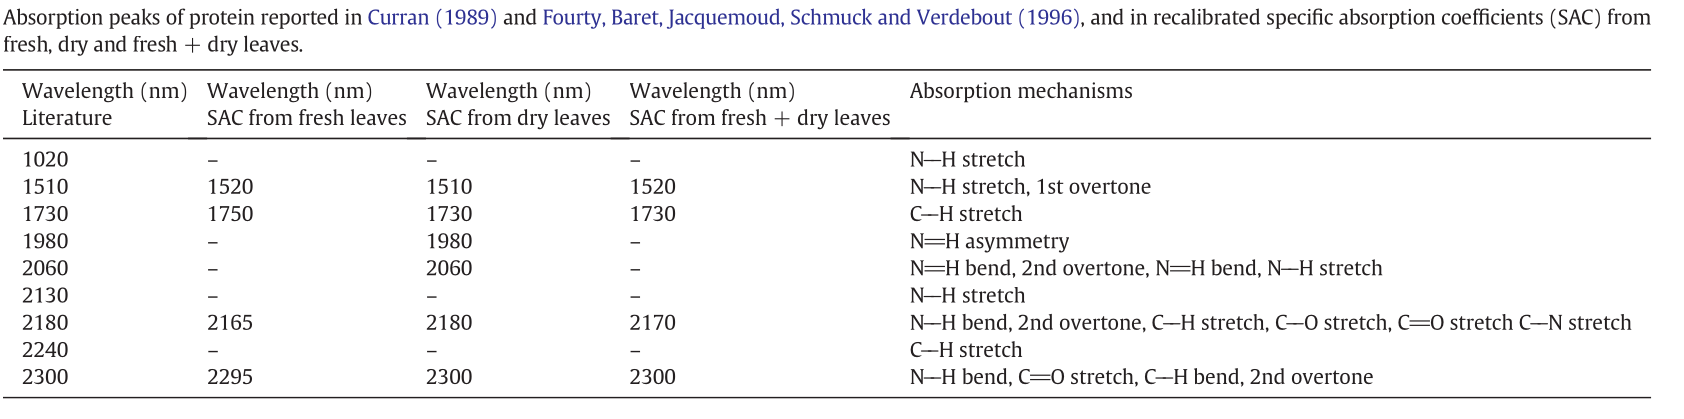
\includegraphics[width=0.95\textwidth]{protein_absorptions.png}\\[8pt]
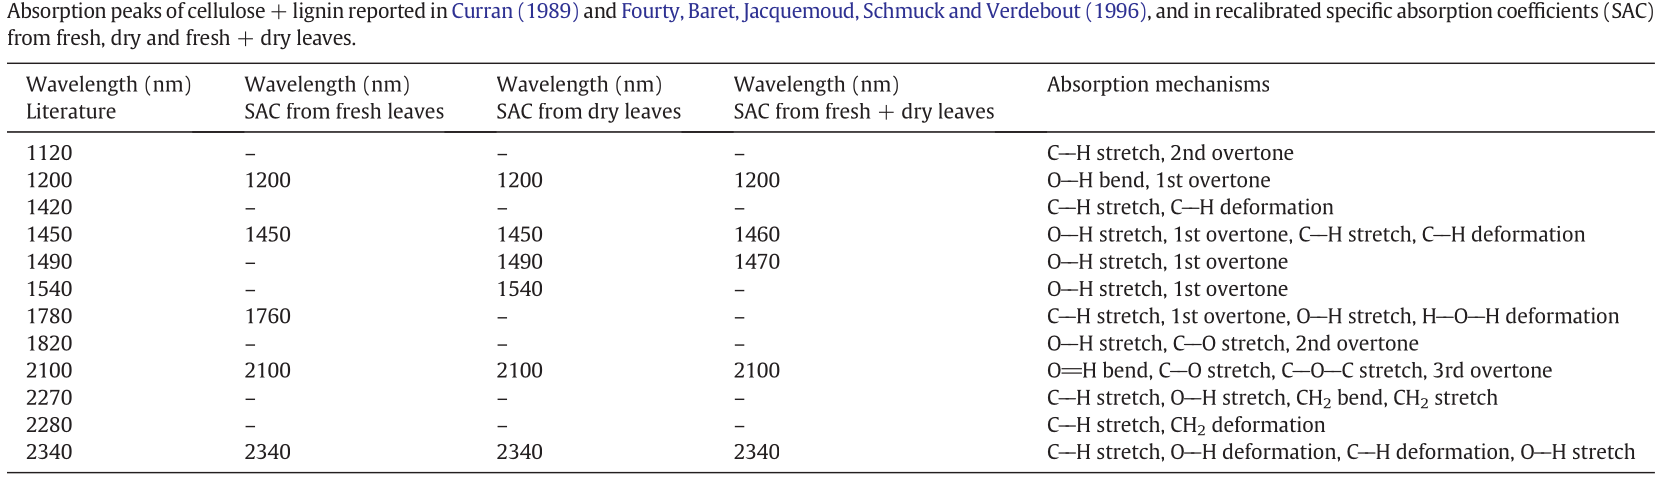
\includegraphics[width=0.95\textwidth]{cellig_absorptions.png}\\[8pt]
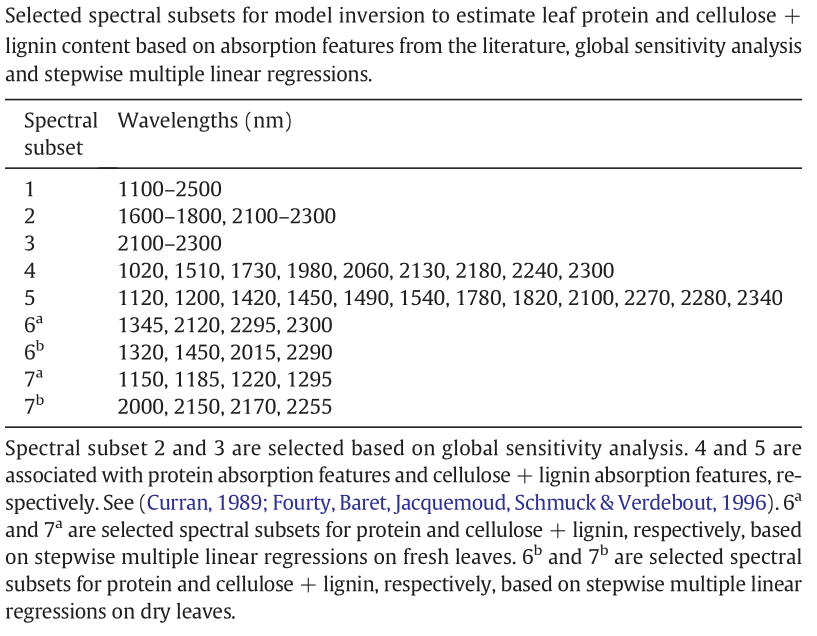
\includegraphics[width=0.6\textwidth]{wavelengths_subsets.png}
\caption{Literature absorption peaks for protein (top) and cellulose +
lignin (middle), and the spectral subsets selected for model inversion
from them (bottom).}
\label{fig:tables}
\end{figure}

\end{document}
